% fundDom.tex      pdflatex ZhCvGo15

% Diffuse globally, compute locally: a cyclist tale
% Tingnan Zhang, Daniel I. Goldman and Predrag Cvitanovi\'c

%\section{Into the fundamental domain}
%\label{s-fundDom}

\begin{figure}[htbp]
  \begin{center}
    (a)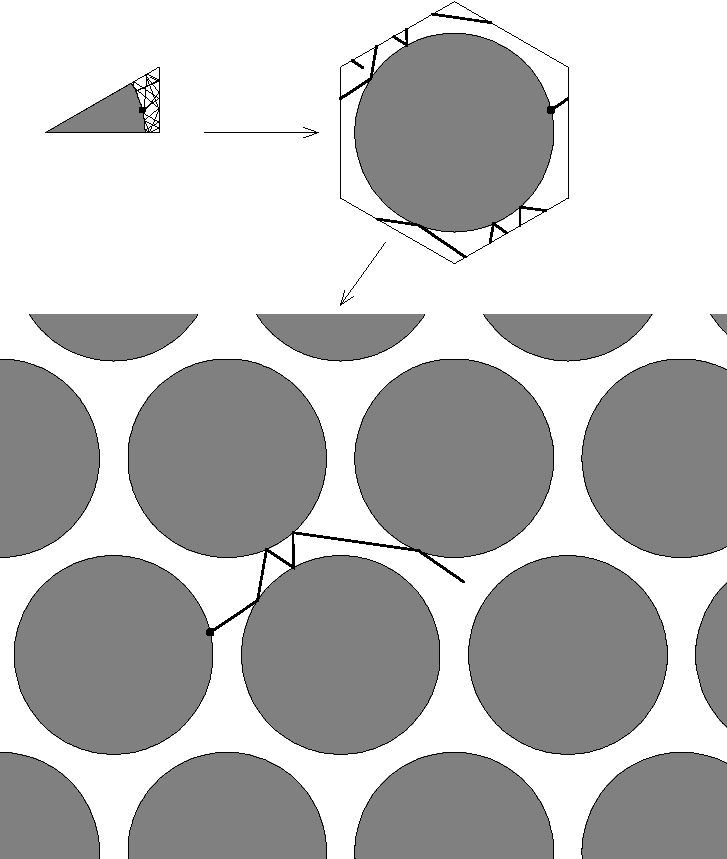
\includegraphics[width=0.45\textwidth]{diffuseSchreiberFig1}
    (b)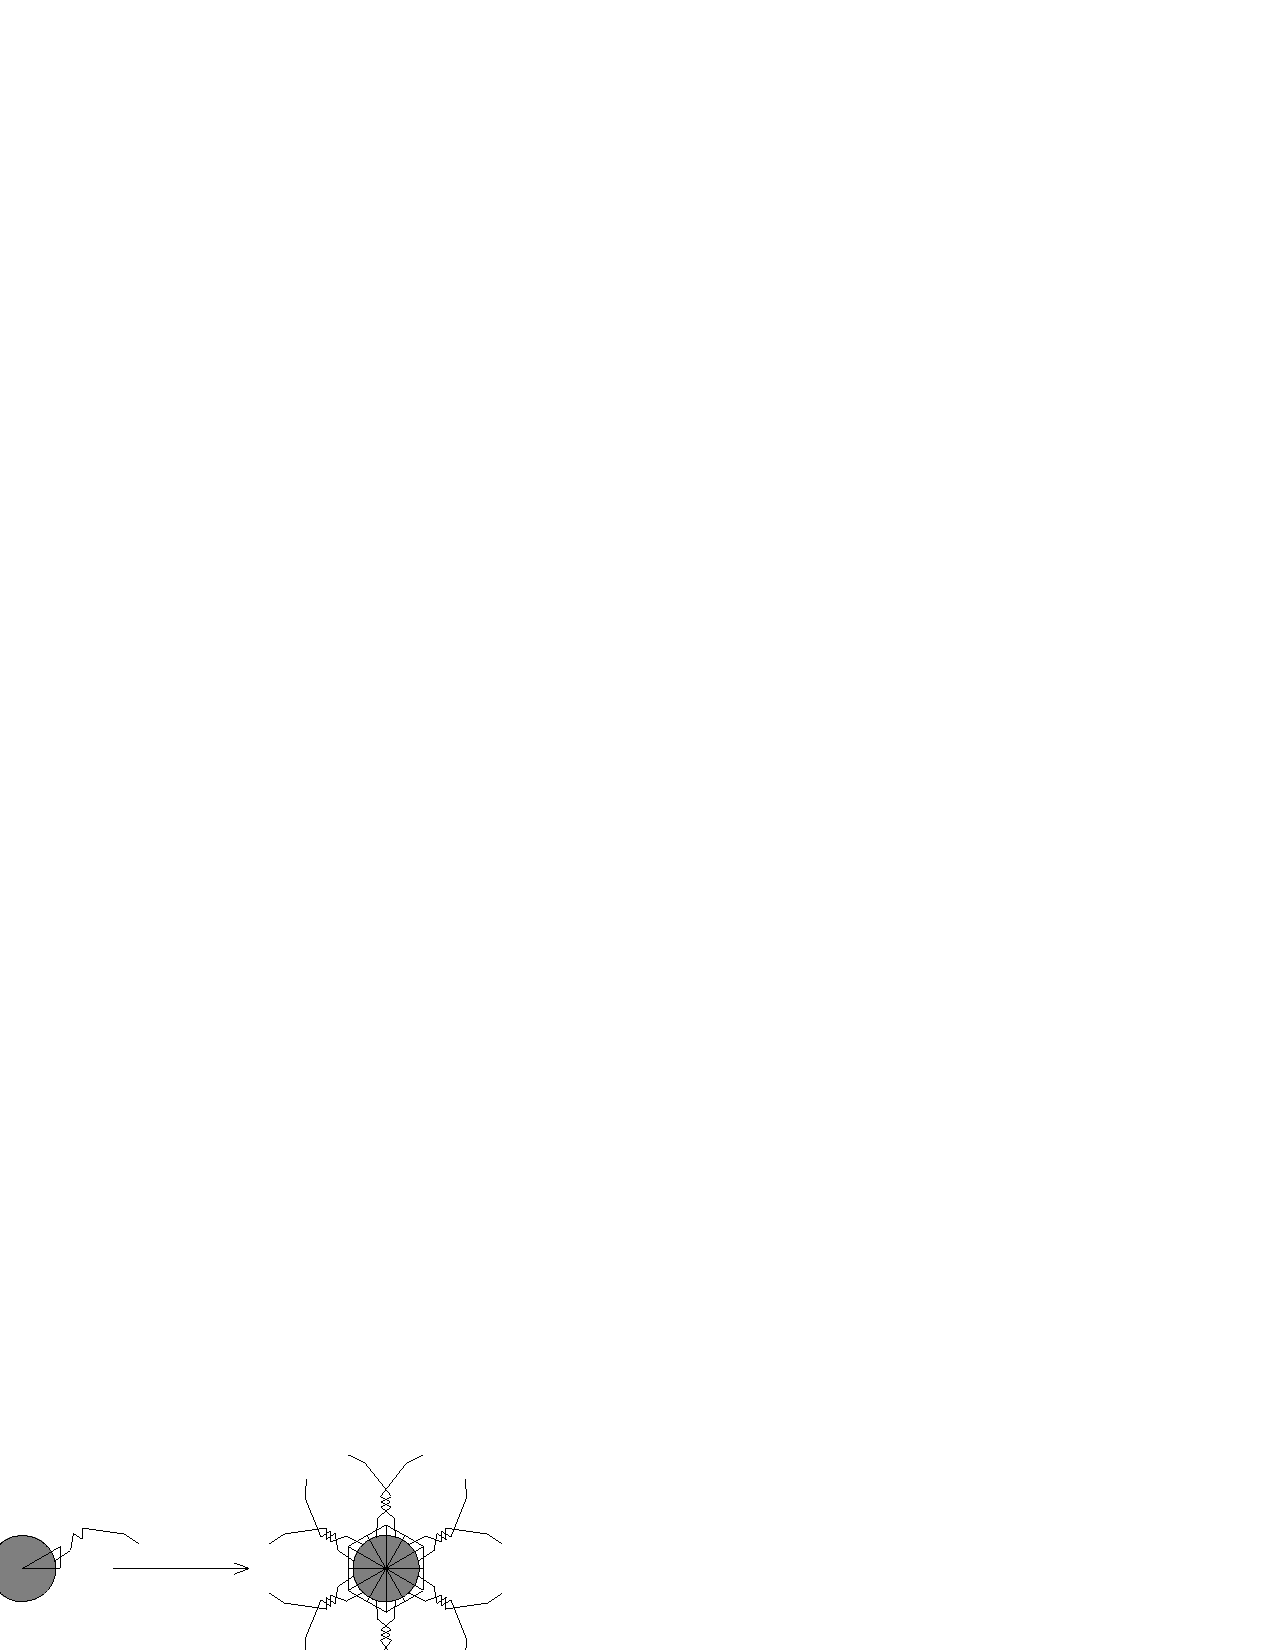
\includegraphics[width=0.45\textwidth]{diffuseSchreiberFig2}
  \end{center}
  \caption[]{\label{fig-schrieberFig12}
  (a) Motion in the fundamental domain (top left), elementary cell (top
      right) and  in full space (bottom).
  (b) An (unwrapped) trajectory (in full  space) and its 12 copies after
      applying point group actions to it.
  }
\end{figure}

%\begin{figure}[htbp]
%  \begin{center}
%    (a)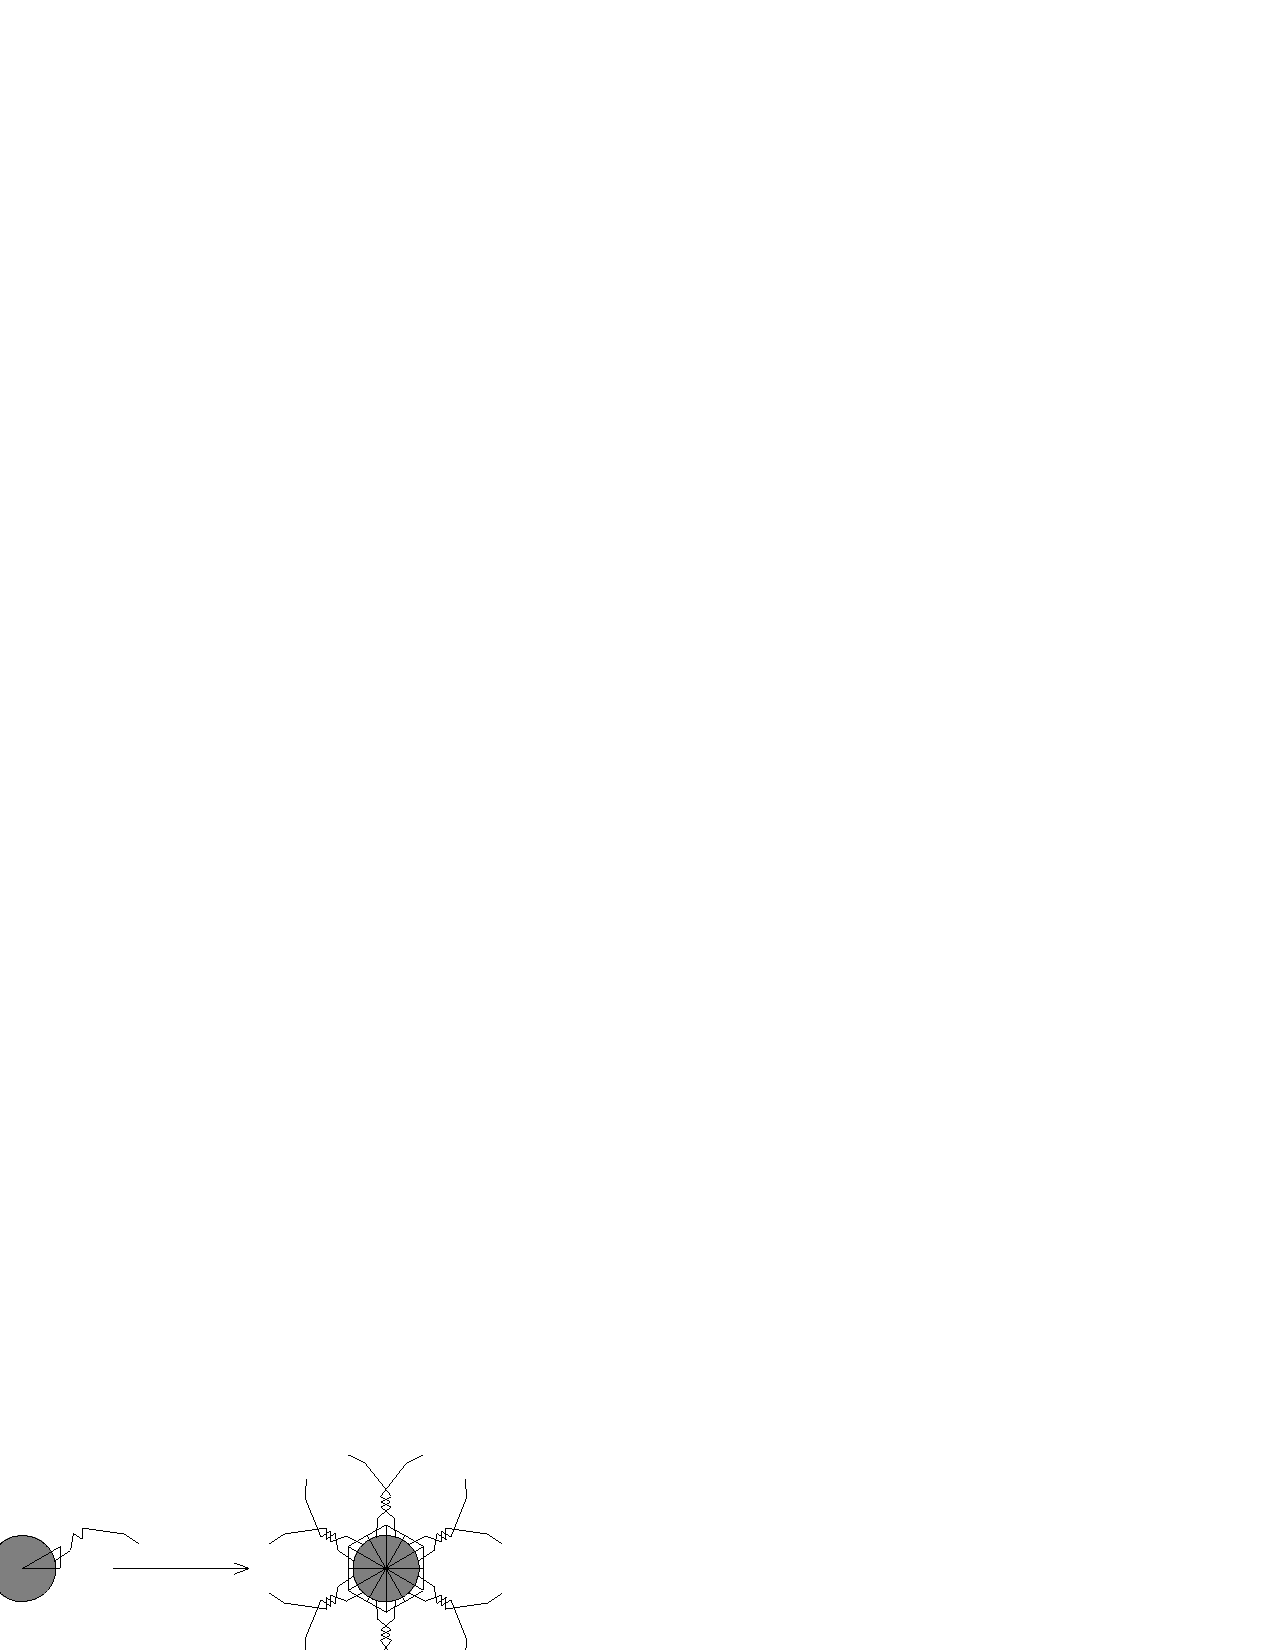
\includegraphics[width=0.45\textwidth]{diffuseSchreiberFig2}
%    (b)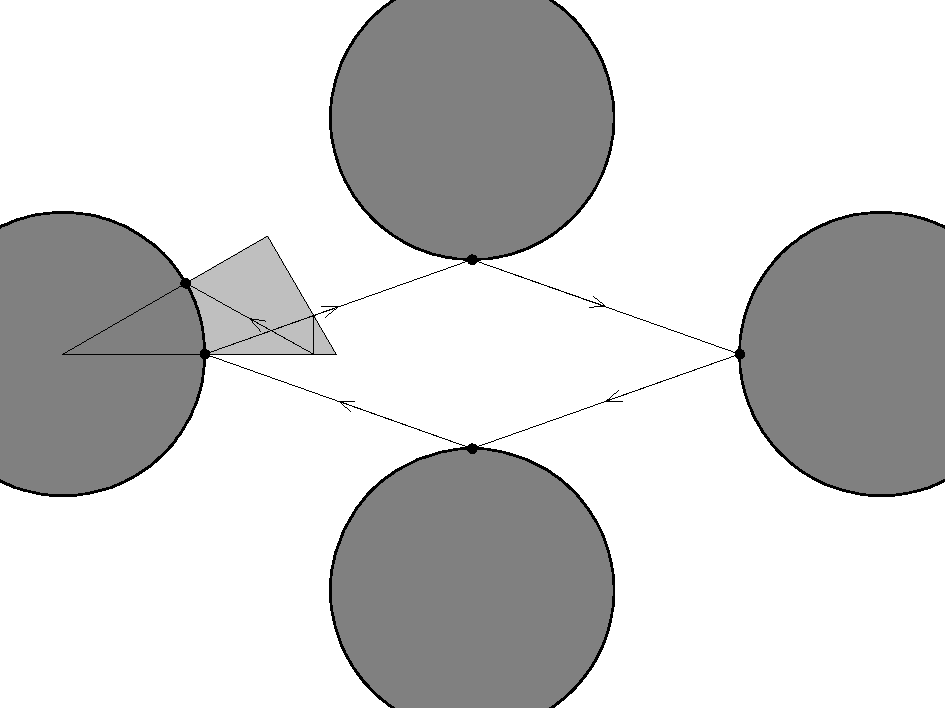
\includegraphics[width=0.45\textwidth]{diffuseSchreiberFig3}
%  \end{center}
%  \caption[]{ \label{fig:schrieberFig23} (a) An (unwrapped) trajectory (in full
%  space) and its 12 copies after applying point group actions to it. (b)
%  Multiplicity of periodic orbits in fundamental domain.}
%\end{figure}

When the scattering array has further discrete symmetries, such as
reflection symmetry, each elementary cell may be built from a {\em
fundamental domain} ${\widetilde \pS}$ by the action of a discrete (not
necessarily abelian) group $G$. The quantity $\tx(t)\,=\,\tflow{t}{\tx}$
denotes the flow in the fundamental domain ${\widetilde \pS}$;
$\tflow{t}{\tx}$ is related to$\flow{}{\tx}$ by a discrete symmetry $g
\in G$ which maps $\tx(t)\in{\widetilde \pS}$ to ${x}(t) \in {\pS}$. The
full $\hM \rightarrow {\widetilde\pS}$ reduction is complicated by the
non-abelian nature of $G$, and will be illustrated in this section in
detail.

\subsection{How point group changes translation}

In the fundamental domain, one has to realize a few facts before
proceeding to the cycle expansion derivation. A point $x$ in the
elementary cell can be uniquely identified by its ``mirror image'' in the
fundamental domain:
\[ %beq
x=g\circ\tx,
\] %eeq
given a group action $g\in G$ the discrete symmetry group. In the
triangular periodic Lorentz gas the underlying point group is $C_{6v}$
(isomorphic to $D_6$), and the hexagonal elementary cell is partitioned
into 12 identical triangular domains. We have to appreciate that the flow
$\hat{\phi}^t$ is G-equivariant under the lattice group symmetry, and
proceed with the argument that the displacement in full space is also
equivariant under the point group symmetry (which is a subset of the
lattice group):
\[ %beq
\hn_t(x)\equiv\hn_t(g\circ\tx)= g\circ\hn_t(\tx).
\] %eeq

We can apply this fact to the displacement associated with a prime
periodic orbit $\tp$ restricted in the fundamental domain.
Let$\tp\equiv\{\tx_0,\tx_1,\ldots,\tx_{N_\tp}\}$, with topological length
$N_\tp$and $\tx_i$ the bouncing points on the orbit. For each flight
(e.g. from $\tx_i$to $\tx_{i+1}$) we denote the associated displacement
in full space $\hn(\tx_i,e)$. However, one has to be careful when adding
the individual displacements together when moving along a fundamental
domain orbit. Unlike in elementary cell, the fundamental domain point
$\tx_i$ does not distinguish in which triangular piece it is. Instead, we
assign a point group element$g_\tp(\tx_{i+1},\tx_{i})$ to keep track of
changes in absolute orientation. We now write the displacement traveled
along the orbit, after finishing a full cycle:
\beq
\hn_{\tp}(\tx_{0})=\sum_{i=0}^{N_\tp-1}\hn(\tx_{i},g_{\tp,\tx_0}(\tx_{i}))
=\sum_{i=0}^{N_\tp-1}g_{\tp,\tx_{0}}(\tx_{i})\circ\hn(\tx_{i},e),
\eeq
where $g_{\tp,\tx_{0}}(\tx_i)=\prod_0^{j-1} g_\tp(\tx_{j+1},\tx_{j})$ is
the accumulated orientation changes along the orbit when starting from
$\tx_{0}$.The displacement now has its dependence on the starting point
we choose. We denote the total group action for the orbit

\bea
h_{\tp}(\tx_i)&\equiv& g_\tp(\tx_{i},\tx_{i-1})\circ\ldots\circ
g_\tp(\tx_{0},\tx_{N_\tp-1})\nonumber\\
&& \circ g_\tp(\tx_{N_\tp-1},\tx_{N_\tp-2})\circ \ldots\circ
g_\tp(\tx_{i+1},\tx_{i}),
\eea
which one can immediately see the connection
$\flow{t_\tp}{\tx_i}=h_{\tp}(\tx_i)\tflow{t_\tp}{\tx_i}$.
Although the group action $h_{\tp}(\tx_i)$ depends on the initial points
on the orbit, it is a property of the orbit's symmetry, and subsequently
all $h_{\tp}(\tx_i), \tx_i\in\tp$ belong to the \emph{same} subgroup of
$G$.

We define the quantity:
\beq
\hat{L}_{\tp}^{r}(\tx_i)\equiv
(e+\hp^{1}(\tx_i)+\cdots+\hp^{r-1}(\tx_i))\cdot\hn_{\tp}(\tx_i),
\label{eq-fdDisplacement}
\eeq
to be the displacement traveled along the orbit $r$ times, starting from
$\tx_i$.  Though one may not appreciate immediately,
\refeq{eq-fdDisplacement} takes care of the rotational symmetry that does
not commute with translation, and we will show that it gives the proper
displacement needed for computing diffusion coefficient in the
fundamental domain.
